\documentclass[
	letterpaper, % Paper size, specify a4paper (A4) or letterpaper (US letter)
	10pt, % Default font size, specify 10pt, 11pt or 12pt
]{CSUniSchoolLabReport}

%----------------------------------------------------------------------------------------
%	REPORT INFORMATION
%----------------------------------------------------------------------------------------

\title{Introduction to RC Circuits \\ Circuits \& Signals \\ EECE2150} % Report title

\author{Michael \textsc{Brodskiy}}

\date{March 20, 2023} % Date of the report

%----------------------------------------------------------------------------------------


\begin{document}

\maketitle % Insert the title, author and date using the information specified above

\begin{center}
	\begin{tabular}{l r}
		Date Performed: & March 13, 2023 \\ % Date the experiment was performed
        Partner: & Juan \textsc{Zapata} \\ % Partner names
		Instructor: & Professor \textsc{Sun} % Instructor/supervisor
	\end{tabular}
\end{center}

\setcounter{section}{-1}

\section{Introduction}

The purpose of this laboratory experimentation is to familiarize oneself with the concept of active pass filters. By integrating a capacitor, in addition to the resistors involved with an operational amplifier, an active pass filter was constructed.

  \section{Part I}

  \subsection{Q1} The constructed virtual circuit appears as follows:

  \begin{figure}[H]
    \centering
    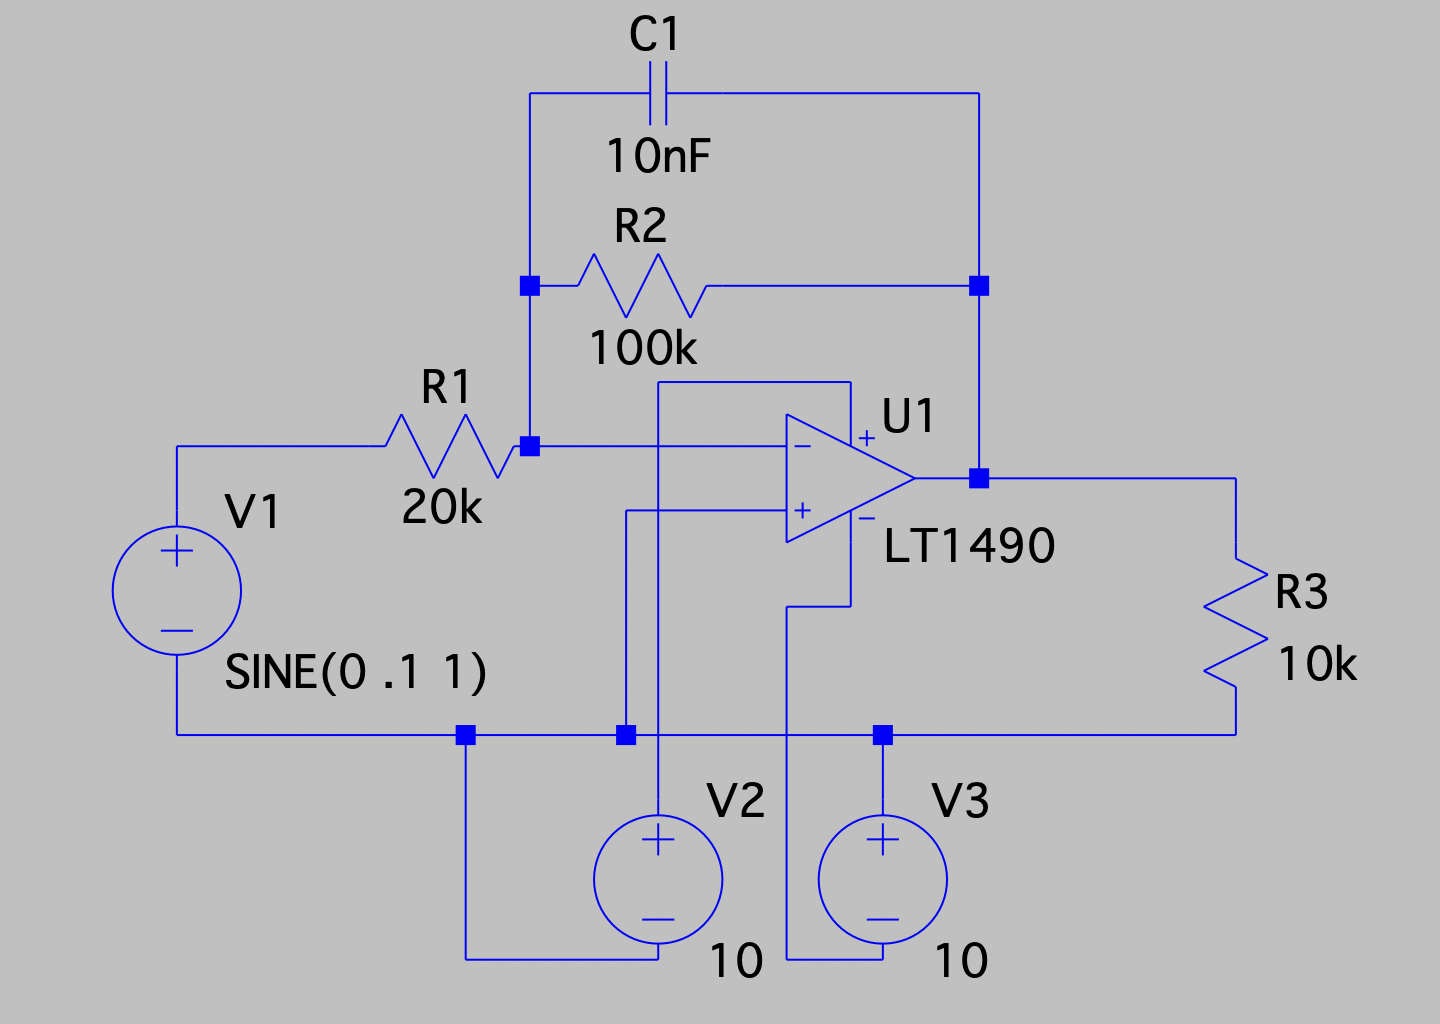
\includegraphics[width=.9\textwidth]{Figures/L10Circ.png}
    \caption{Constructed Active Filter}
    \label{fig:1}
  \end{figure}

  \subsection{Q2} The found value of the cutoff frequency, $f_c$, is $159[\si{\hertz}]$. This is roughly the expected value, as the expected value may be calculated using: $\frac{1}{2\pi\cdot 100[\si{\kilo\ohm}]\cdot10[\si{\nano\farad}]}=159.155[\si{\hertz}]$

  \subsection{Q3} Though the output voltage is 5 times its previous value, the cutoff frequency remains the same, meaning that the transfer function remains the same

  \subsection{Q4} The input is a square wave, while the output is exponential and rounded to a point. The output looks as it does because the capacitor is charging. Because of the negative amplifier, the capacitor discharges when the source is positive, and charges when negative. In terms of the Fourier transform, the frequency peaks appear at roughly the same values for inputs and outputs, but the output has much higher peaks. The input is much more consistent in its values.

\section{Conclusion}

Overall, this laboratory experiment introduced us to the concept of active filters through transform and Fourier analysis. In this manner, the concept of active filters was easier to grasp through real-world examples.

\end{document}
